\documentclass[11pt,a4paper]{article}
\usepackage{fontspec}
\setmainfont{TeX Gyre Pagella}
\newfontfamily\headfont{Inter}[UprightFont=*-ExtraBold,BoldFont=*-ExtraBold,Extension=.otf,Path=/usr/share/fonts/opentype/inter/]
\usepackage[a4paper,margin=2.3cm]{geometry}
\usepackage{graphicx,booktabs,float,caption,array,xcolor,longtable}
\usepackage{xurl}
\usepackage[hidelinks]{hyperref}
\usepackage{titlesec}
\usepackage[round]{natbib}
\usepackage{setspace}
\setstretch{1.05}
\renewcommand{\topfraction}{0.9}
\renewcommand{\bottomfraction}{0.8}
\renewcommand{\textfraction}{0.1}
\renewcommand{\floatpagefraction}{0.75}
\setlength{\parindent}{0pt}
\setlength{\parskip}{0.55em}
\titleformat{\section}{\headfont\Large}{\thesection}{0.8em}{}
\titleformat{\subsection}{\headfont\large}{\thesubsection}{0.8em}{}
\captionsetup{font=small,labelfont=bf}
\urlstyle{same}
\hypersetup{pdftitle={Could Your Town Fit in Its Stadium?},pdfauthor={Tristan Hotham}}

\begin{document}
\begin{center}
{\Large\bfseries Could Your Town Fit in Its Stadium?\par}
\vspace{0.4em}
{\large Sports venues bigger than the towns they stand in, from Wikidata\par}
\vspace{1.2em}
{\large Tristan Hotham\par}
\vspace{0.3em}
{\small Independent researcher\\
ORCID: 0000-0003-4931-9349\\
DOI: https://doi.org/10.5281/zenodo.24087795\par}
\vspace{0.8em}
2026
\end{center}

\begin{quote}
\small
\begin{center}\textbf{Abstract}\end{center}
I compare the capacity of 11,658 sports venues of 1,000 seats or more in Wikidata with the population of the place each stands in. A first pass finds 321 venues with more seats than their place has people, but most are artefacts of how places are recorded: of 375 venues read by eye, 133 stand in a district or suburb of a larger city, 17 have a wrong population, are not real venues or have been demolished, 3 are placed in a county or borough, 2 are unresolved, and 33 are real towns whose capacity or population needed correcting (50.1\% in all). After correction, 190 venues in 48 countries are bigger than their town, 73 of them at least twice. The largest ratios belong to a minor-league ballpark in the village of Sauget, Illinois (42.5 seats per resident), a Gaelic games ground in the Irish town of Clones (15.4), a football ground in Aixovall, Andorra, and American college and professional stadiums in small municipalities, led by Beaver Stadium (9.9 times College Township). Racecourses, motor circuits and winter sports venues reach higher still (Oakbank Racecourse 80.9, the Indianapolis Motor Speedway 18.4) and are reported separately. In Britain and Ireland, Gaelic games county grounds lead (St Tiernach's Park, Clones, 15.4; Semple Stadium, Thurles, 5.6); the highest English Football League ratio is Bolton Wanderers' ground at Horwich (1.4). By country, Wikidata's venues amount to 311 seats per 1,000 people in Qatar and 210 in Ireland, against 106 in the United Kingdom.

\textbf{Keywords:} stadiums; sports venues; capacity; small towns; Gaelic games; college football; Wikidata; data quality
\end{quote}

\section{Introduction}
Some towns are famous for a ground far too big for them: the American college town that triples in size on a Saturday, the Irish county town whose Gaelic football ground holds several times its population, the motor-racing village that fills for one weekend. This paper asks which sports venues in the world are bigger than the towns they stand in, using the capacities and locations recorded in Wikidata \citep{vrandecic2014}. The ratio of capacity to population is simple; the difficulty is the denominator. A venue's ``located in'' place may be a county, a big city, a ward or a suburb, and the head of a ranking by ratio collects exactly the cases where it is the wrong one. The method is therefore a simple ratio plus a complete reading by eye of every case at the head of the ranking, with all decisions released.

\section{Data}
A Wikidata query (run with QLever; \citealt{bast2017}) returned venues that are instances of sports venue (Q1076486) or its subclasses with a capacity (P1083) of at least 1,000, with coordinates, country, located-in places (P131) with their populations (P1082), tenants (P466) and the number of sitelinks. The rows come one per combination of values; I aggregated them to 11,658 venues in 210 countries, 10,284 of which have a population for at least one located-in place. Country populations are Natural Earth estimates \citep{naturalearth}. For the UK I also used Wikidata's list of settlements with population and type. For the cases quoted in the text I checked capacities against current published figures (Wikipedia and club pages), and for Irish towns, many of which have no population in Wikidata or only an older census figure, I took the 2022 census population of the census town \citep{cso2022}. Each correction and its source is recorded in \texttt{code/overrides.csv}.

\section{Methods}
\textbf{Capacity and population.} Where several values are recorded, I take the largest capacity (204 venues have more than one, often an old record crowd alongside today's figure) and the largest population of the place. Where a venue has several located-in places (332 venues), I take the one with the smallest population, which is usually the town rather than the county or region. The first pass uses Wikidata's values as they stand; the hand corrections described above are applied after the checks.

\textbf{Kind and sport.} Wikidata's venue types are not in the extract, so the kind of venue (stadium, arena, racecourse, motor circuit, winter sports venue, bullring, showground, tennis or water sports venue) is guessed from the name, and the sport from the name and the tenants' names. Stadiums and arenas form the main ranking; the others are reported separately, since they fill only on a few days a year.

\textbf{UK cross-check.} For British venues I found the nearest town, city or village in the Wikidata settlement list within 4 km. It agrees with the located-in place for only 38.5\% of venues, often because it lands on a neighbouring village; filling missing populations from it produced nonsense (a village of a few hundred for Hillsborough), so it is kept only as a column in the data.

\textbf{Checks by eye.} Every venue with a ratio of 1 or more (321) and the British and Irish venues down to 0.4 were read by eye and given a verdict in \texttt{code/overrides.csv}: a town in its own right (with a corrected capacity or population where needed), a district or suburb of a larger city, a wrong population or venue or a demolished venue, a county or borough, or unsure. A place counts as a town if it is a municipality, township, commune or village in its own right, even if it adjoins a big city; a suburb or ward that is only part of a city does not.

\section{Results}
\subsection{Venues bigger than their towns}
After the checks, 190 venues in 48 countries have more seats than their town has people; 165 of them are stadiums or arenas and 73 have at least two seats per resident. Figure~\ref{fig:scatter} shows all stadiums and arenas against their town's population, and Table~\ref{tab:world} the fifteen with the highest ratio. The largest is GCS Ballpark in Sauget, Illinois, an industrial village of 141 with a minor-league ballpark of 6,000 seats (42.5 per resident), followed by St Tiernach's Park, the Monaghan county ground in Clones (29,000 for 1,885 people, 15.4), the Estadi Comunal d'Aixovall in Andorra (12.5), the Xanthi FC Arena in the village of Pigadia, unused since 2022 (11.5), Beaver Stadium (9.9) and MetLife Stadium in East Rutherford (8.2).

\begin{figure}[tbp]\centering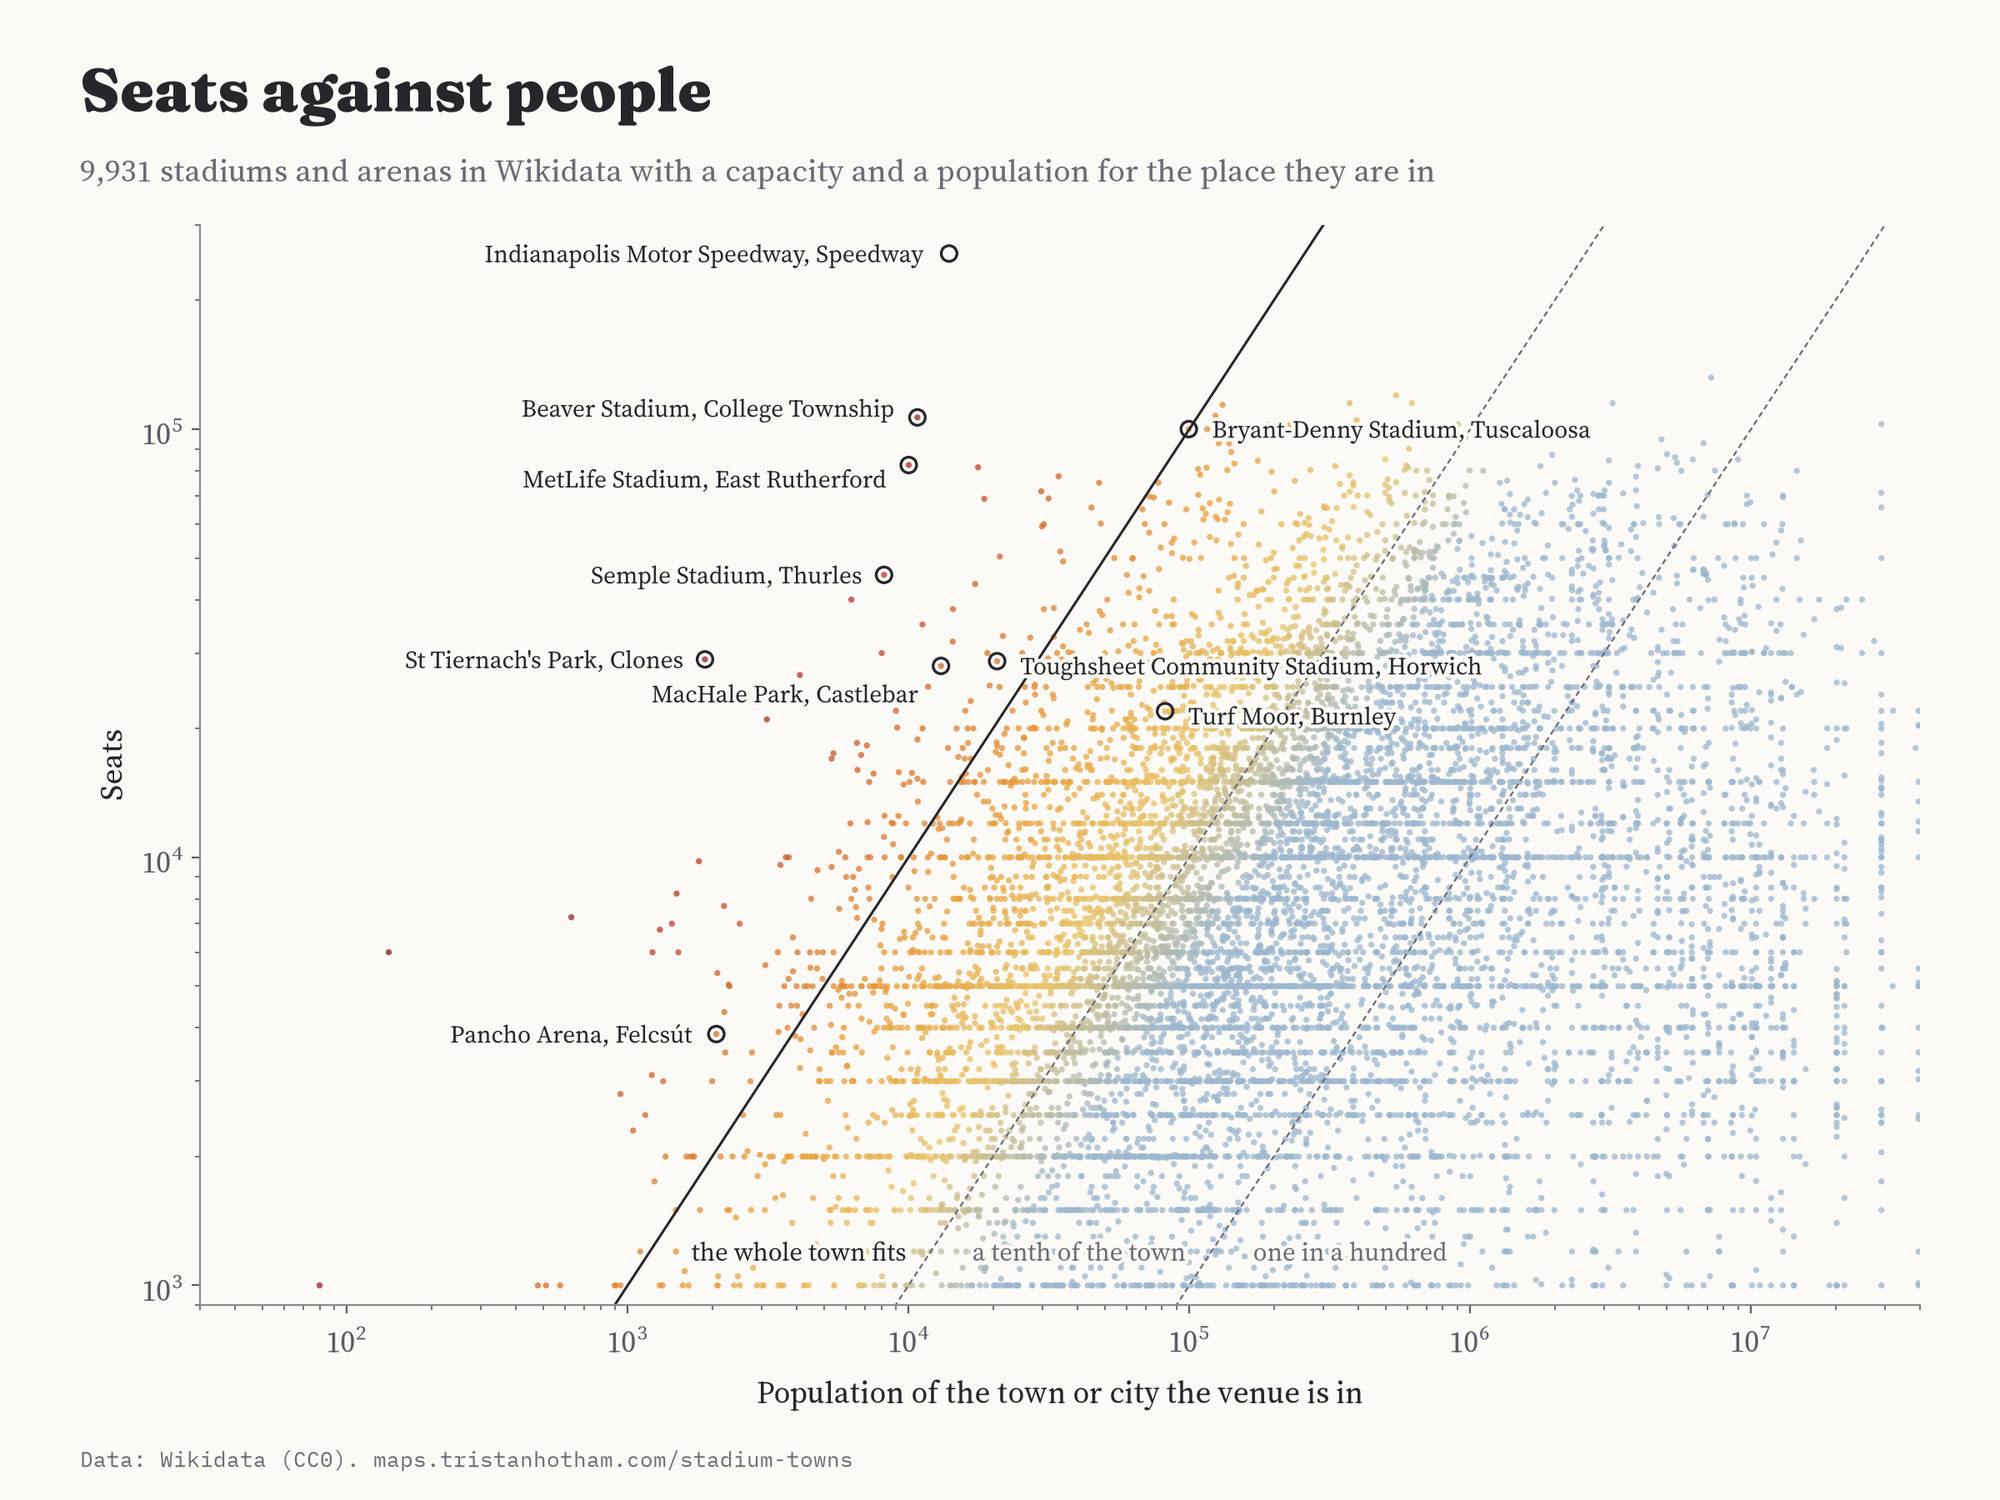
\includegraphics[width=0.95\linewidth]{f_scatter.png}\caption{Capacity against the population of the place, for stadiums and arenas (log scales). Above the solid line the whole town fits.}\label{fig:scatter}\end{figure}

\begin{table}[tbp]\centering\small\caption{The fifteen stadiums and arenas with the most seats per resident of their town (checked by eye).}\label{tab:world}\begin{tabular}{rp{4.6cm}p{4.2cm}rrr}\toprule & Venue & Town & Seats & People & Seats a head\\\midrule
1 & GCS Ballpark & Sauget, US & 6,000 & 141 & 42.55\\
2 & St Tiernach's Park & Clones, Ireland & 29,000 & 1,885 & 15.38\\
3 & Estadi Comunal d'Aixovall & Aixovall, Andorra & 1,000 & 80 & 12.50\\
4 & Xanthi FC Arena & Pigadia, Greece & 7,244 & 630 & 11.50\\
5 & Beaver Stadium & College Township, US & 106,572 & 10,762 & 9.90\\
6 & MetLife Stadium & East Rutherford, US & 82,500 & 10,022 & 8.23\\
7 & Stadler Stadion & Akasztó, Hungary & 21,000 & 3,131 & 6.71\\
8 & Stade Saint-Symphorien & Longeville-lès-Metz, France & 26,671 & 4,102 & 6.50\\
9 & Howard J. Lamade Stadium & South Williamsport, US & 40,000 & 6,261 & 6.39\\
10 & Semple Stadium & Thurles, Ireland & 45,690 & 8,185 & 5.58\\
11 & Aigeira Municipal Stadium & Aigeira, Greece & 8,230 & 1,494 & 5.51\\
12 & Doubleday Field & Cooperstown, US & 9,791 & 1,794 & 5.46\\
13 & Nuova Valascia & Quinto, Switzerland & 6,775 & 1,302 & 5.20\\
14 & Svangaskarð & Nes Municipality, Faeroe Is. & 6,000 & 1,226 & 4.89\\
15 & Aughrim County Ground & Aughrim, Ireland & 7,000 & 1,437 & 4.87\\
\bottomrule\end{tabular}\end{table}

American college football supplies many of the largest cases (Table~\ref{tab:college}): Clemson (4.6), Notre Dame (2.3), Stanford (2.4), and Bryant-Denny Stadium in Tuscaloosa, which at 100,077 seats would hold the whole city (1.00). Professional football's suburban stadiums appear because they stand in small municipalities: MetLife in East Rutherford (Giants Stadium, which stood beside it, was demolished in 2010), Gillette Stadium in Foxborough (3.7). In European football, the leaders are grounds in villages and small communes near the cities they serve: Aixovall, Xanthi, the abandoned Stadler Stadion in Akasztó, Saint-Symphorien in Longeville-lès-Metz, the Pancho Arena in Felcsút (1.9).

\begin{table}[tbp]\centering\small\caption{American college stadiums bigger than their town.}\label{tab:college}\begin{tabular}{rp{4.6cm}p{4.2cm}rrr}\toprule & Venue & Town & Seats & People & Seats a head\\\midrule
1 & Beaver Stadium & College Township, US & 106,572 & 10,762 & 9.90\\
2 & Memorial Stadium, Clemson & Clemson, US & 81,500 & 17,681 & 4.61\\
3 & Warren McGuirk Alumni Stadium & Hadley, US & 17,000 & 5,325 & 3.19\\
4 & Stanford Stadium & Stanford, US & 50,424 & 21,150 & 2.38\\
5 & Notre Dame Stadium & Clay Township, US & 77,622 & 34,235 & 2.27\\
6 & Mountaineer Field at Milan Puskar Stadium & Morgantown, US & 60,000 & 30,347 & 1.98\\
7 & Kidd Brewer Stadium & Boone, US & 30,000 & 19,092 & 1.57\\
8 & Spartan Stadium & East Lansing, US & 75,005 & 47,741 & 1.57\\
9 & Kelly/Shorts Stadium & Mount Pleasant, US & 32,885 & 21,688 & 1.52\\
10 & SECU Stadium & College Park, US & 51,802 & 34,740 & 1.49\\
\bottomrule\end{tabular}\end{table}

\begin{figure}[tbp]\centering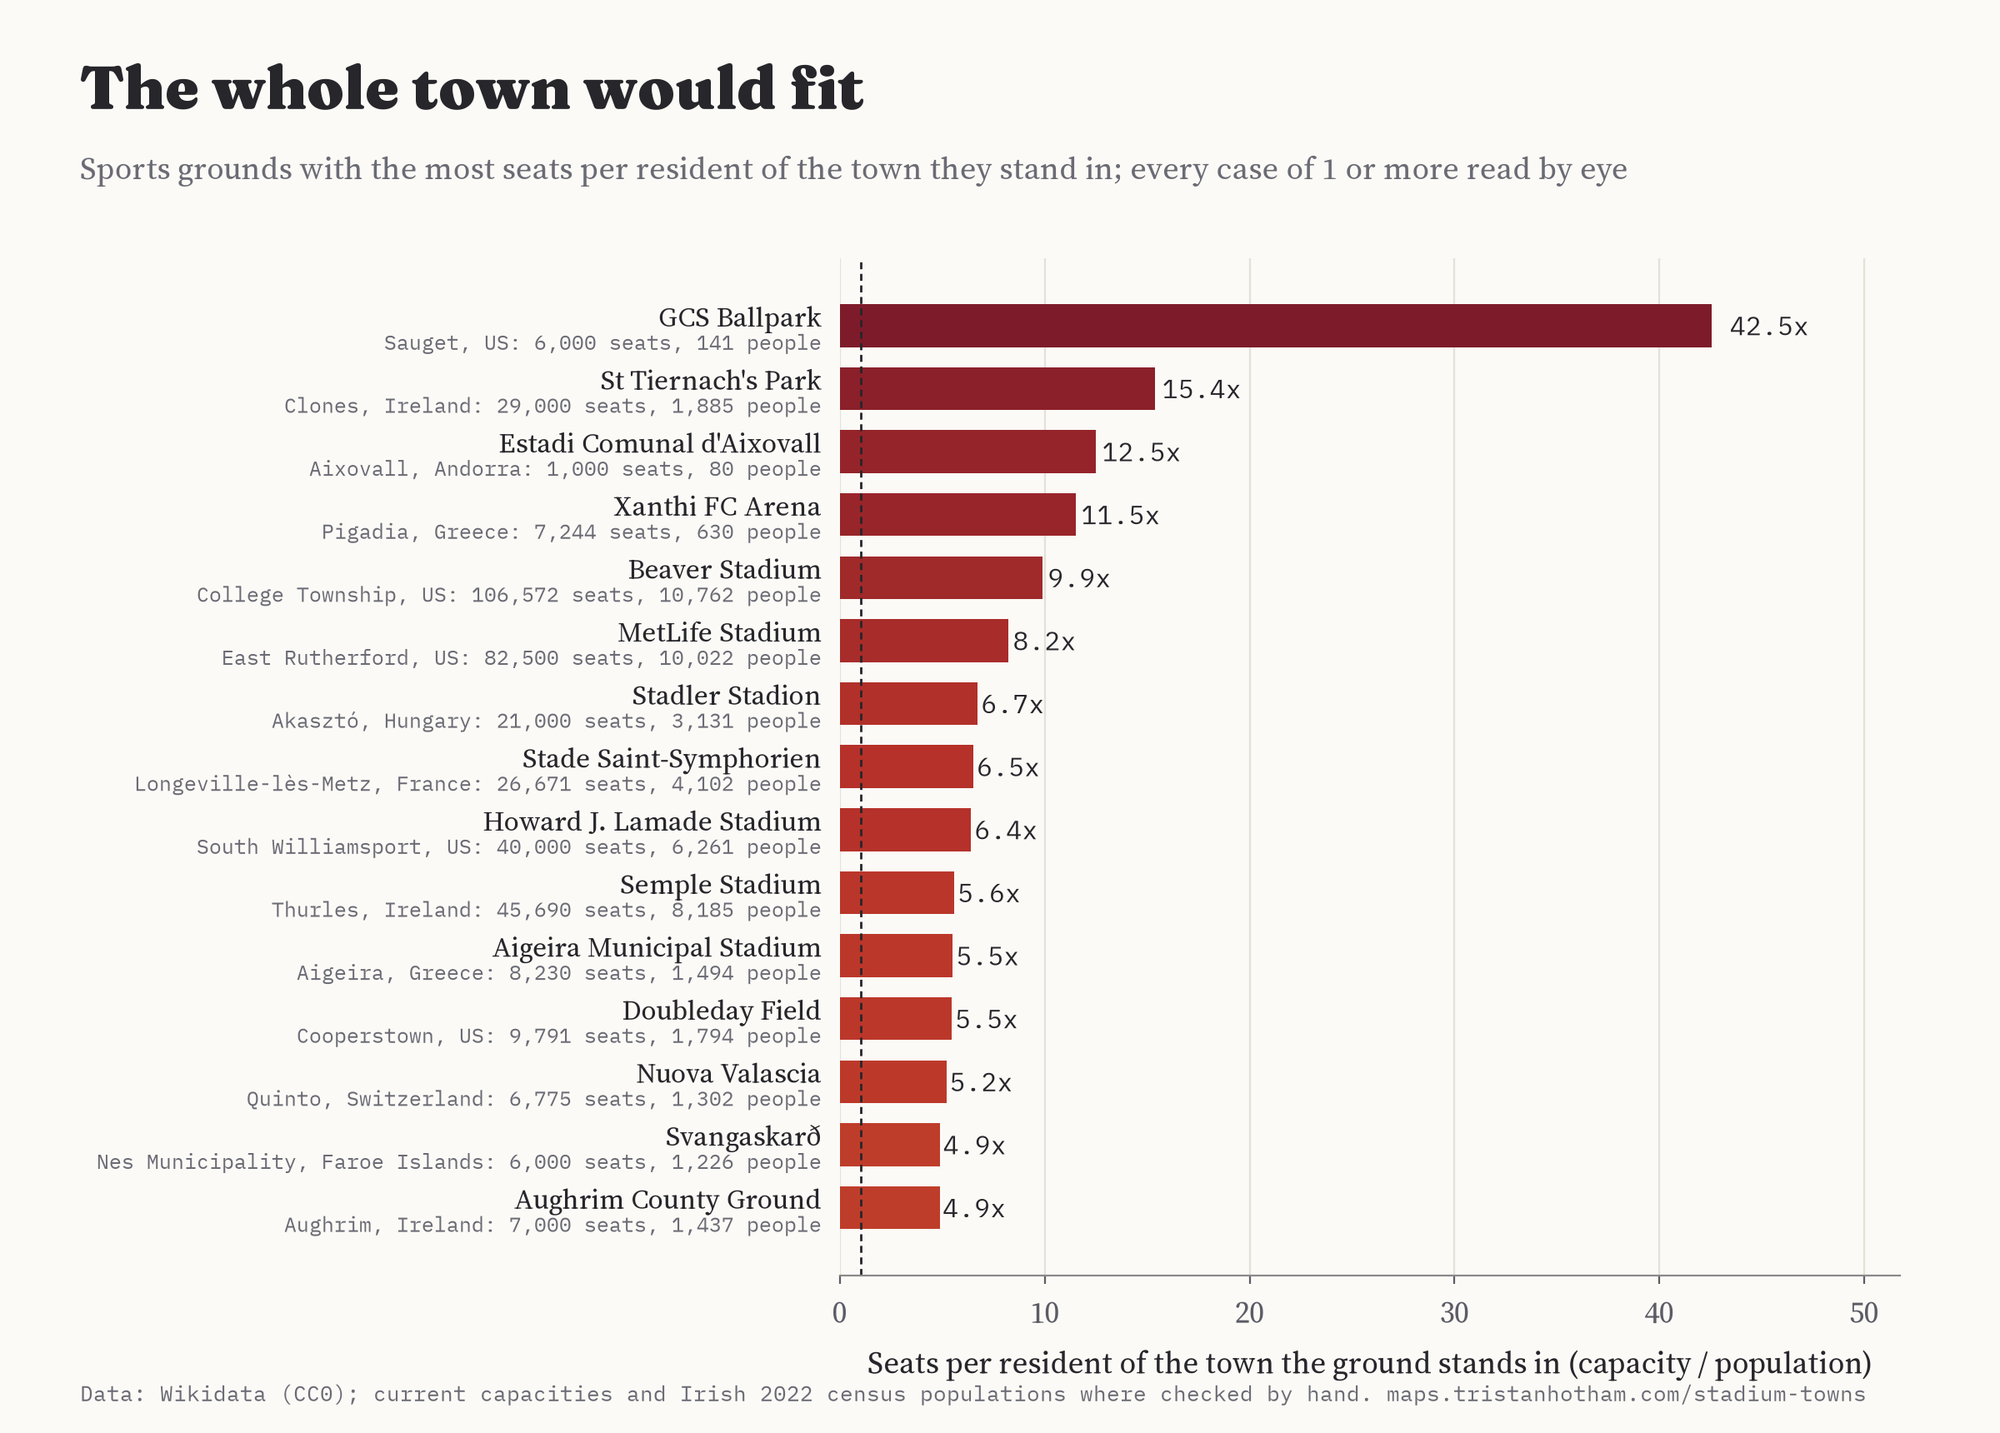
\includegraphics[width=0.95\linewidth]{f_world.png}\caption{Stadiums and arenas with the most seats per resident of their town.}\label{fig:world}\end{figure}

\subsection{Venues for a few days a year}
Racecourses, motor circuits and winter sports venues reach the highest ratios (Figure~\ref{fig:kinds}): Oakbank Racecourse in the Adelaide Hills (70,000 for 865 people, 80.9), the Indianapolis Motor Speedway in the town of Speedway (18.4), the cross-country ski stadium at Lago di Tesero (16.9) and Chantilly Racecourse (2.8). Wikidata records few racecourses and circuits as sports venues with a capacity, so these lists are short.

\begin{figure}[tbp]\centering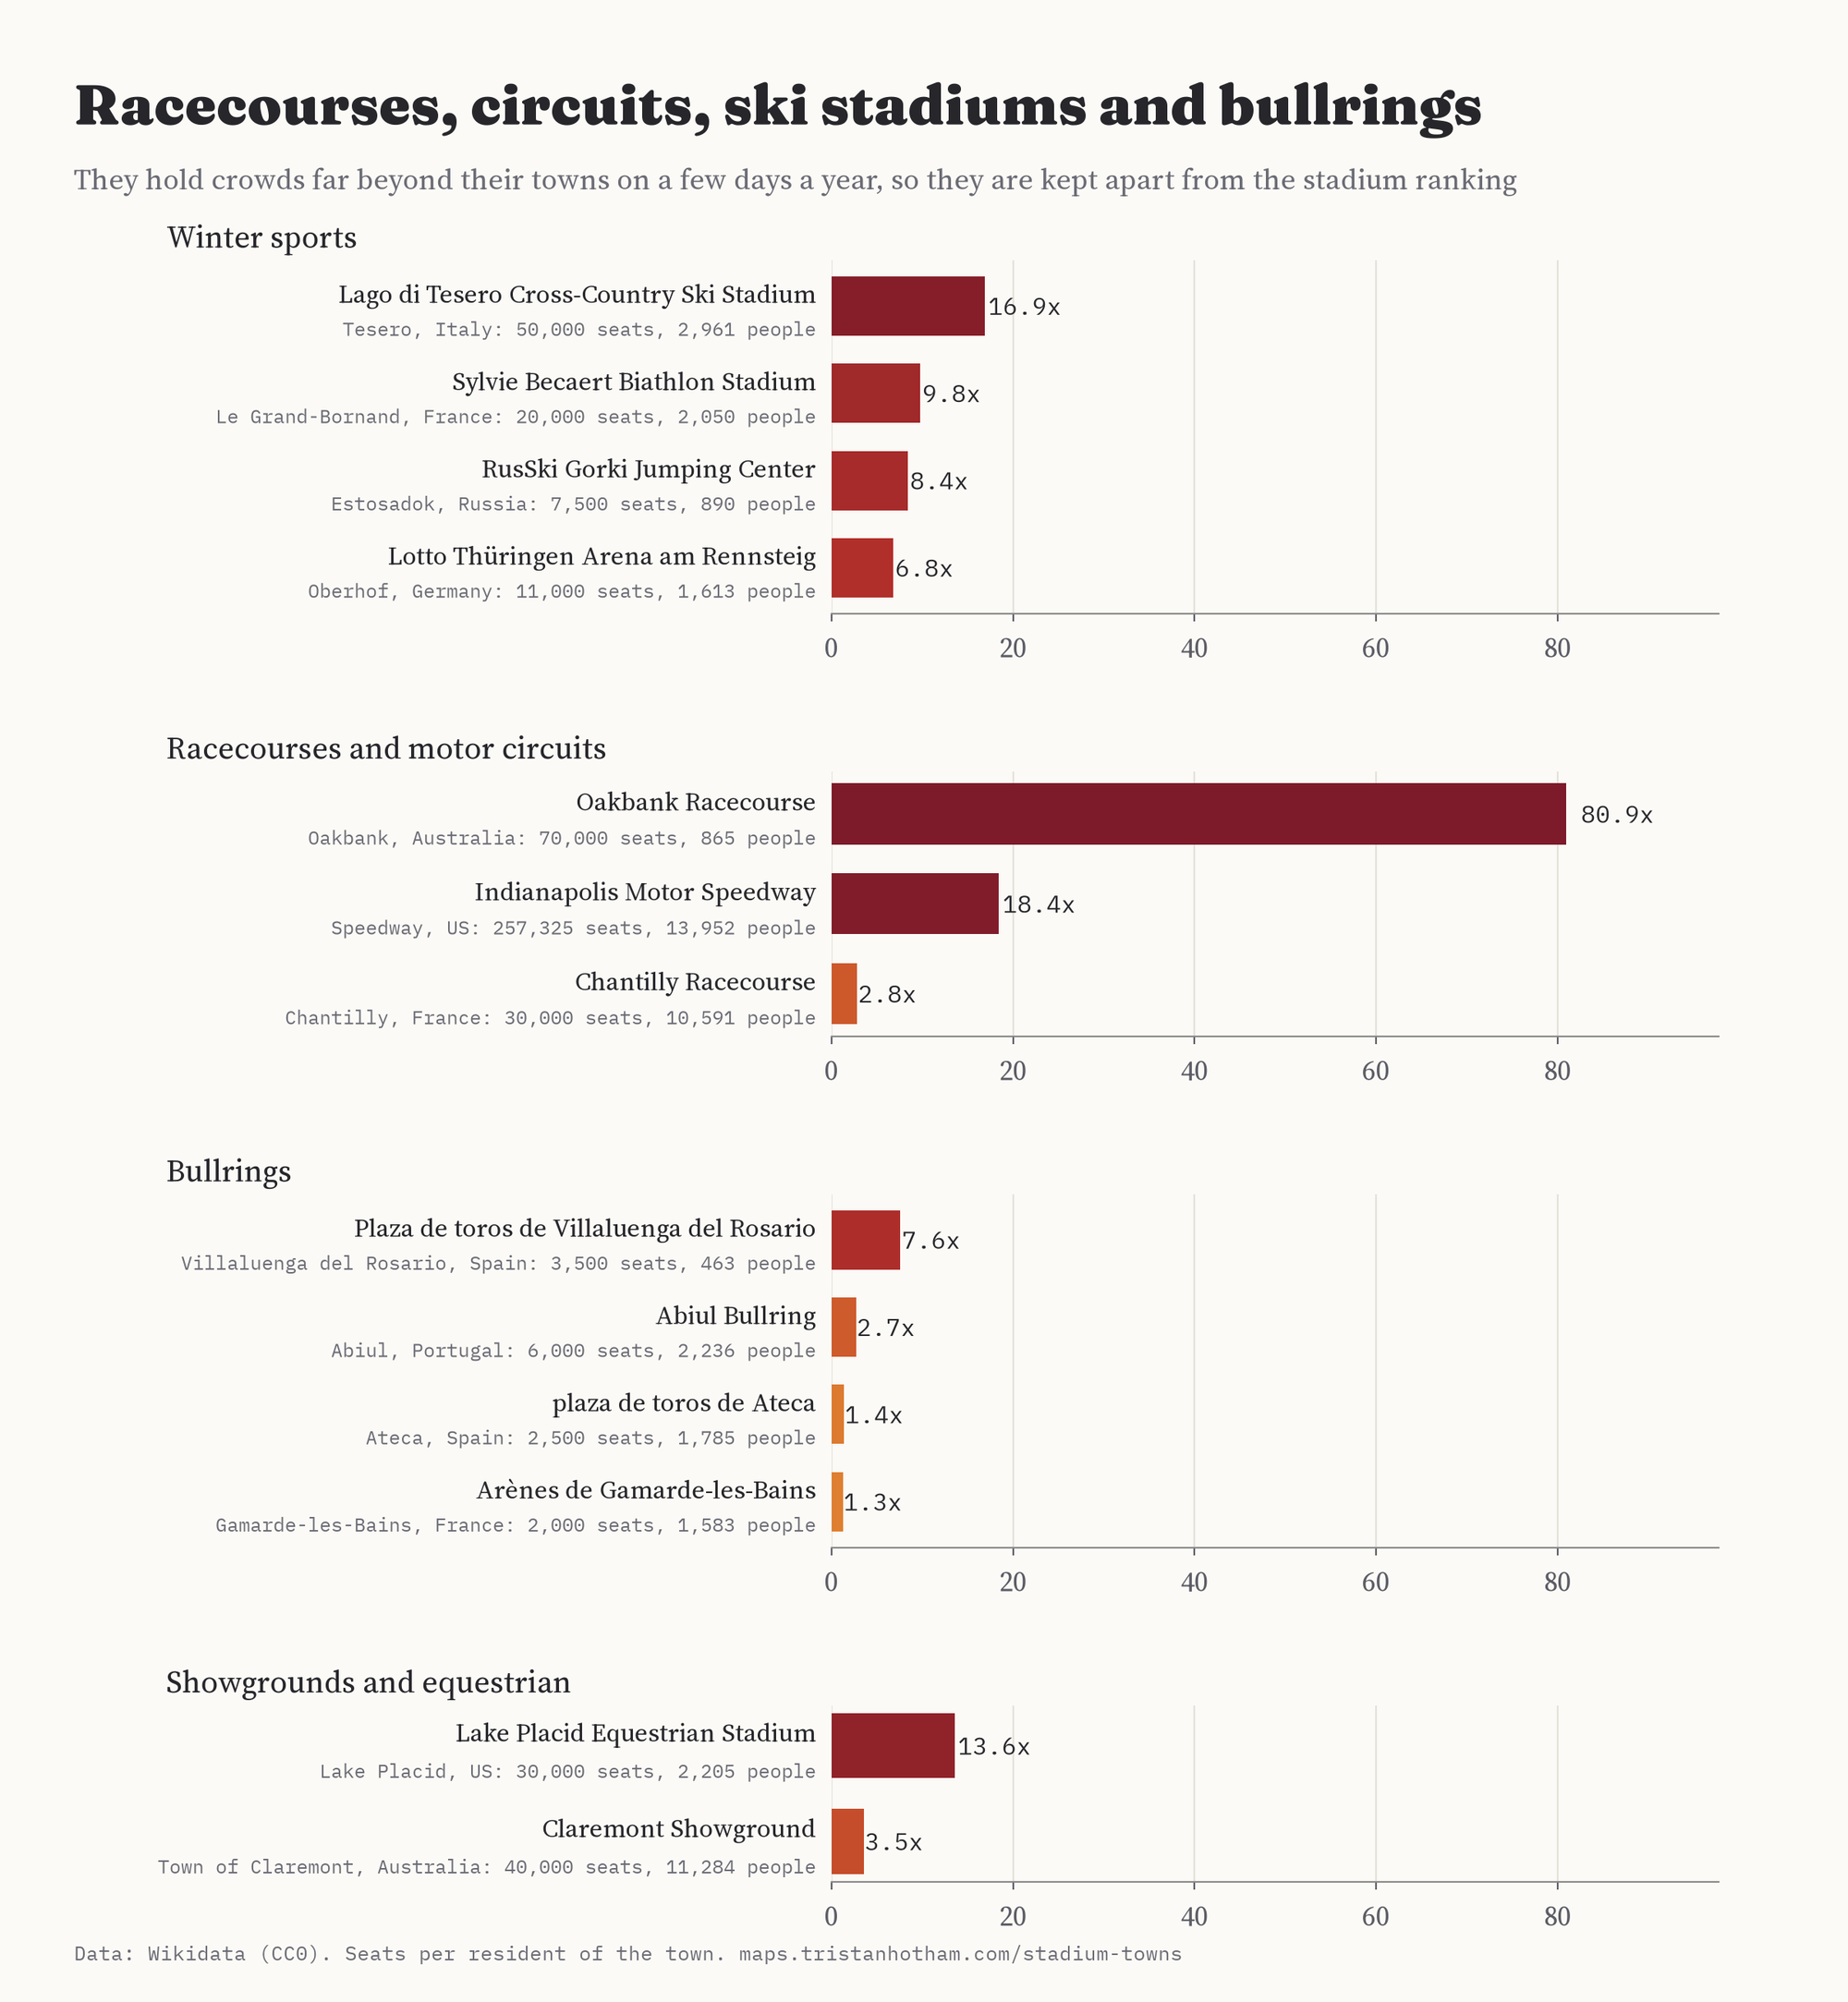
\includegraphics[width=0.85\linewidth]{f_kinds.png}\caption{Winter sports venues, racecourses and circuits, bullrings and showgrounds with the most seats per resident.}\label{fig:kinds}\end{figure}

\subsection{Britain and Ireland}
Irish Gaelic games county grounds dominate the list for these islands (Figure~\ref{fig:ukie}, Table~\ref{tab:ukie}): St Tiernach's Park in Clones (15.4), Semple Stadium in Thurles (5.6), the Aughrim County Ground (4.9), then MacCumhail Park in Ballybofey, Dr Hyde Park in Roscommon, O'Garney Park in Sixmilebridge, Fitzgerald Stadium in Killarney, MacHale Park in Castlebar (2.1) and Breffni Park in Cavan, all above two. Several of these were missing from a ranking built on Wikidata alone: it has no population for Thurles, Clones or Cavan and places Fitzgerald Stadium and Dr Hyde Park in their counties. In Northern Ireland, Brewster Park in Enniskillen and the Athletic Grounds in Armagh exceed their towns' populations. In Britain the highest ratios are Northwich Victoria's Victoria Stadium in Wincham (2.2), the Crabble Athletic Ground in the parish of River (1.7), Maes Tegid in Bala (1.5) and Bolton Wanderers' stadium in Horwich (1.4), the only Football League ground among them. The famous big-city grounds have no town ratio because they stand in districts: Anfield, Wembley and the London Stadium in Stratford are all among the 133 district verdicts. Burnley's Turf Moor seats 0.27 of the town.

\begin{figure}[tbp]\centering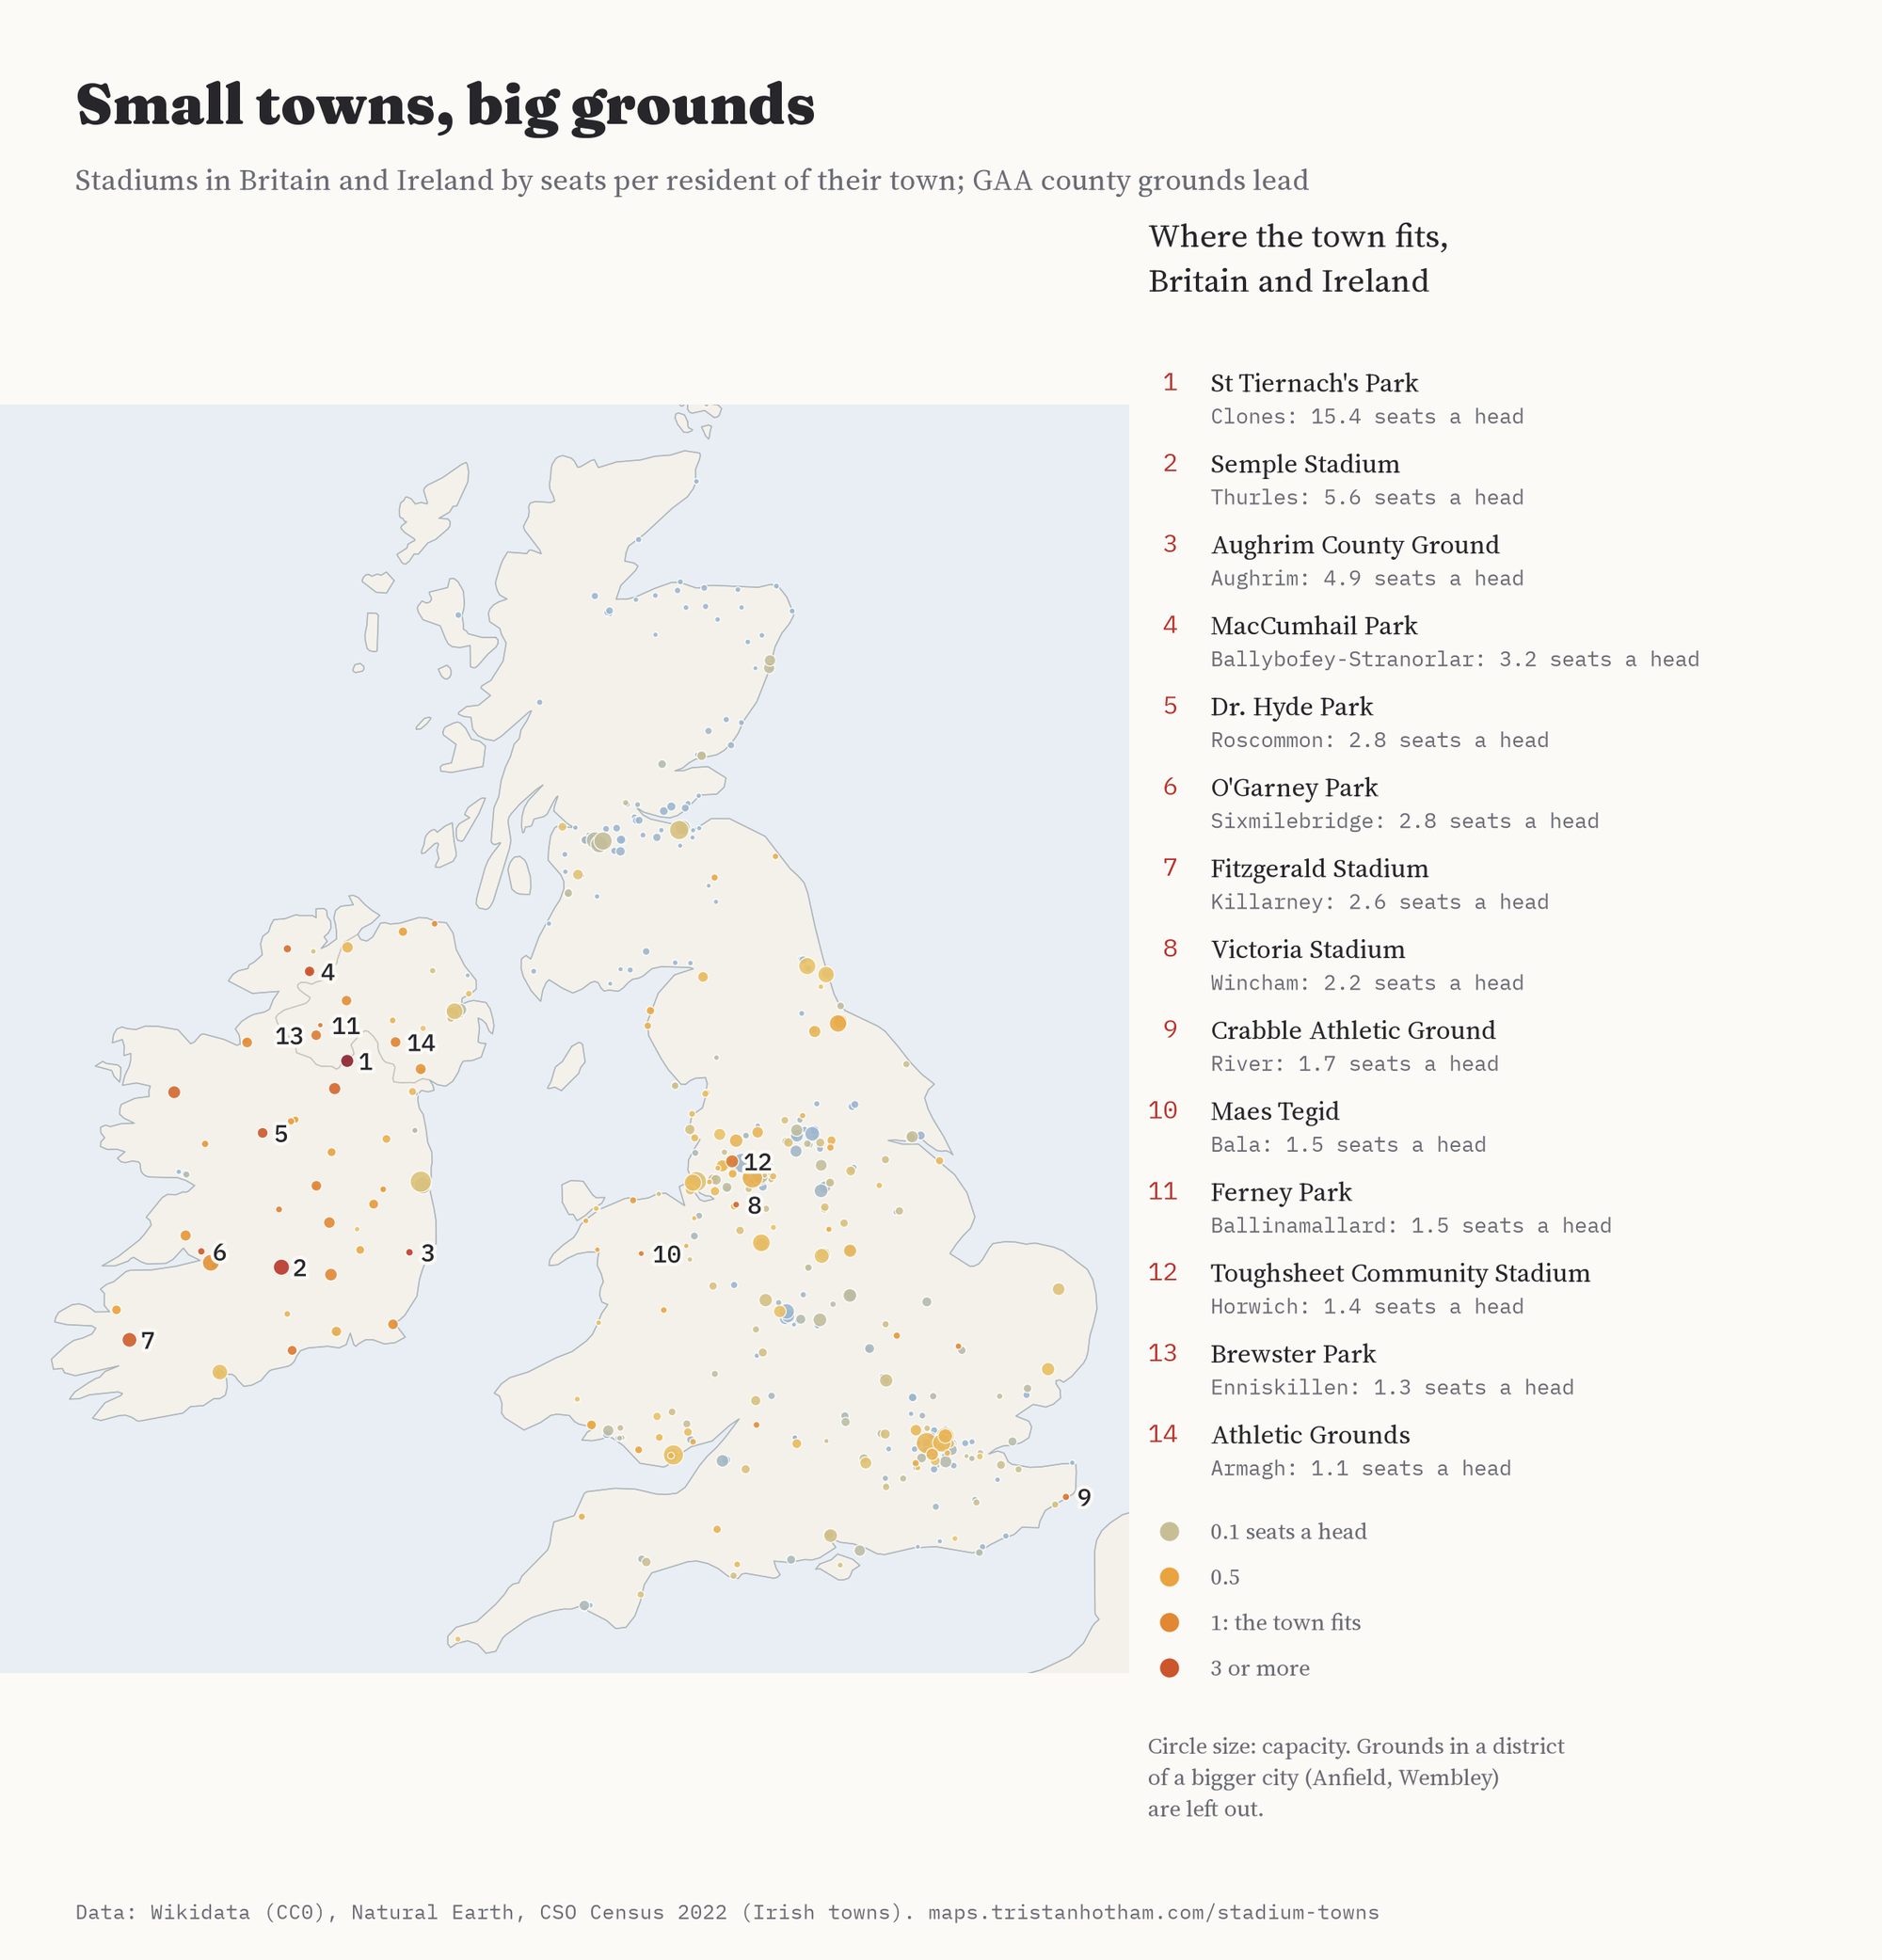
\includegraphics[width=0.85\linewidth]{f_ukie.png}\caption{Stadiums in Britain and Ireland by seats per resident of their town.}\label{fig:ukie}\end{figure}

\begin{table}[tbp]\centering\small\caption{Britain and Ireland: grounds with the most seats per resident of their town.}\label{tab:ukie}\begin{tabular}{rp{4.6cm}p{4.2cm}rrr}\toprule & Venue & Town & Seats & People & Seats a head\\\midrule
1 & St Tiernach's Park & Clones, Ireland & 29,000 & 1,885 & 15.38\\
2 & Semple Stadium & Thurles, Ireland & 45,690 & 8,185 & 5.58\\
3 & Aughrim County Ground & Aughrim, Ireland & 7,000 & 1,437 & 4.87\\
4 & MacCumhail Park & Ballybofey-Stranorlar, Ireland & 17,500 & 5,406 & 3.24\\
5 & Dr. Hyde Park & Roscommon, Ireland & 18,500 & 6,555 & 2.82\\
6 & O'Garney Park & Sixmilebridge, Ireland & 7,000 & 2,507 & 2.79\\
7 & Fitzgerald Stadium & Killarney, Ireland & 38,000 & 14,412 & 2.64\\
8 & Victoria Stadium & Wincham, United Kingdom & 5,045 & 2,289 & 2.20\\
9 & MacHale Park & Castlebar, Ireland & 28,000 & 13,054 & 2.14\\
10 & Crabble Athletic Ground & River, United Kingdom & 6,500 & 3,876 & 1.68\\
11 & Maes Tegid & Bala, United Kingdom & 3,000 & 1,999 & 1.50\\
12 & Ferney Park & Ballinamallard, United Kingdom & 2,000 & 1,364 & 1.47\\
13 & Toughsheet Community Stadium & Horwich, United Kingdom & 28,723 & 20,690 & 1.39\\
14 & Brewster Park & Enniskillen, United Kingdom & 18,000 & 13,823 & 1.30\\
\bottomrule\end{tabular}\end{table}

\subsection{By sport and by country}
Of the 165 stadiums and arenas bigger than their town, 71 are football (soccer) grounds by the names and tenants, 21 American football, 4 baseball and 15 Gaelic games; 44 could not be assigned. Summing every venue in a country and dividing by its population (Figure~\ref{fig:seats}) gives 310.9 seats per 1,000 people in Qatar, 210.0 in Ireland (second of 110 countries of over a million people with ten or more venues), 105.9 in the United Kingdom (rank 11) and 88.8 in the United States (rank 19). These figures measure Wikidata's coverage as much as stadium building: China (3.6) and India (2.1) are certainly undercounted.

\begin{figure}[tbp]\centering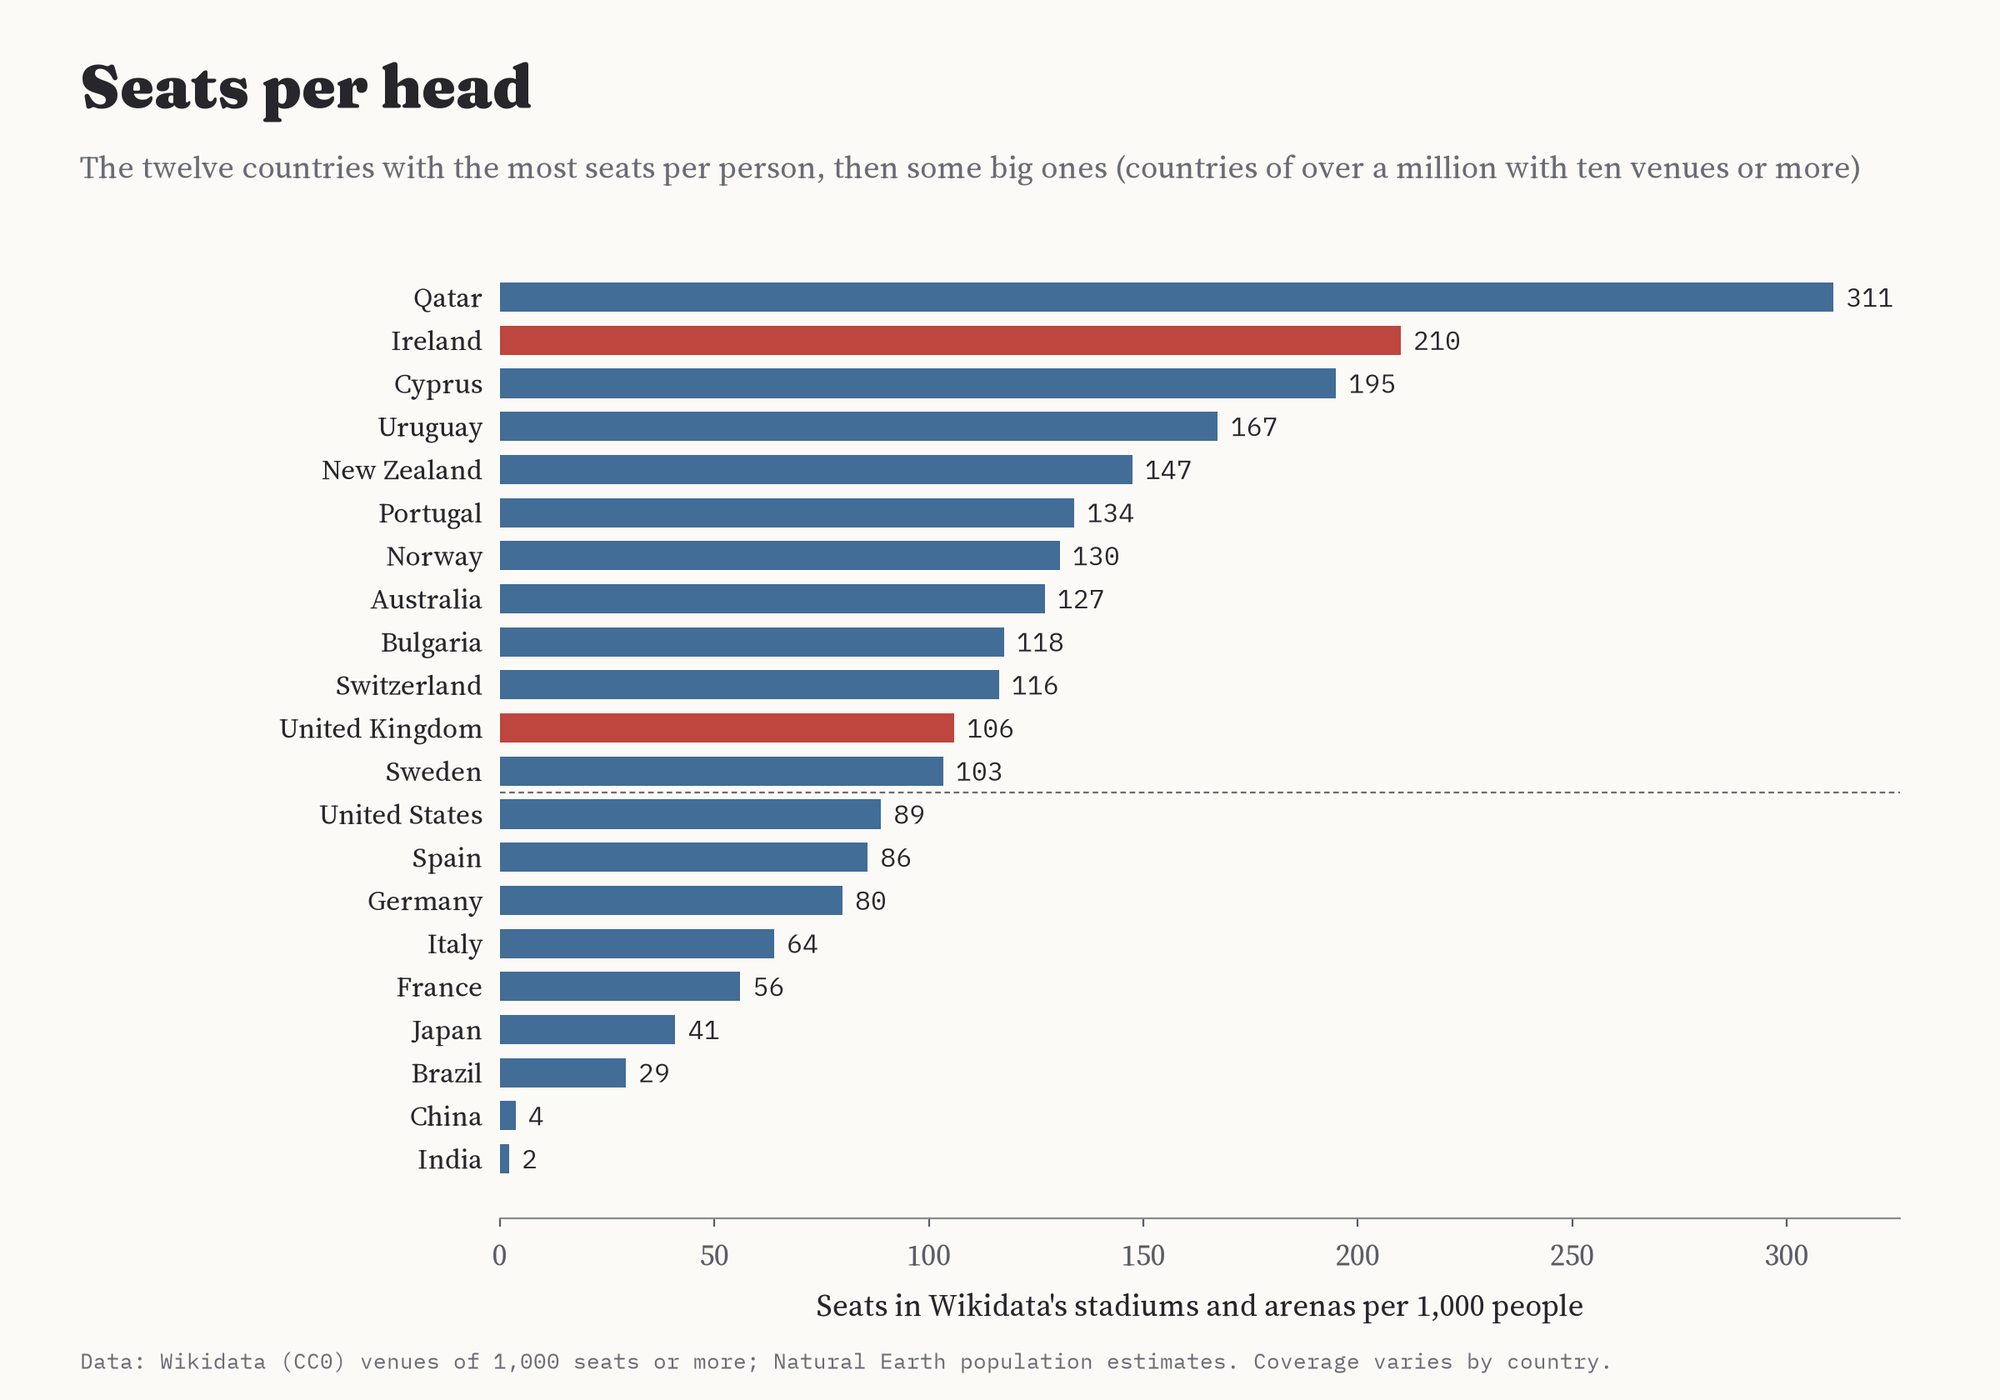
\includegraphics[width=0.85\linewidth]{f_seats.png}\caption{Seats in Wikidata's venues per 1,000 people by country.}\label{fig:seats}\end{figure}

\subsection{What the checks found}
Of the 375 venues read by eye, 220 were kept (Figure~\ref{fig:checks}). The rest show the usual traps of a located-in property. Australian grounds are placed in their suburb (Moore Park for the Sydney Showground, 28 residents), European grounds in a city district (Stockum for Düsseldorf's arena, La Maternitat i Sant Ramon for Camp Nou), Indian grounds in a ward, American college stadiums in a county (Lafayette County for Ole Miss). Some populations are wrong (Kotor given as 562, Maspalomas as 94), some venues were never built (the Kirkby Project, New Trafford) and 6 were demolished long ago (Giants Stadium, Foxboro Stadium, the Pontiac Silverdome among them). Of the kept venues, 33 needed a correction: MacHale Park's recorded 42,000 is an old figure (about 28,000 today), Notre Dame Stadium has held 77,622 since 2017, and many Irish towns lack a population.

\begin{figure}[tbp]\centering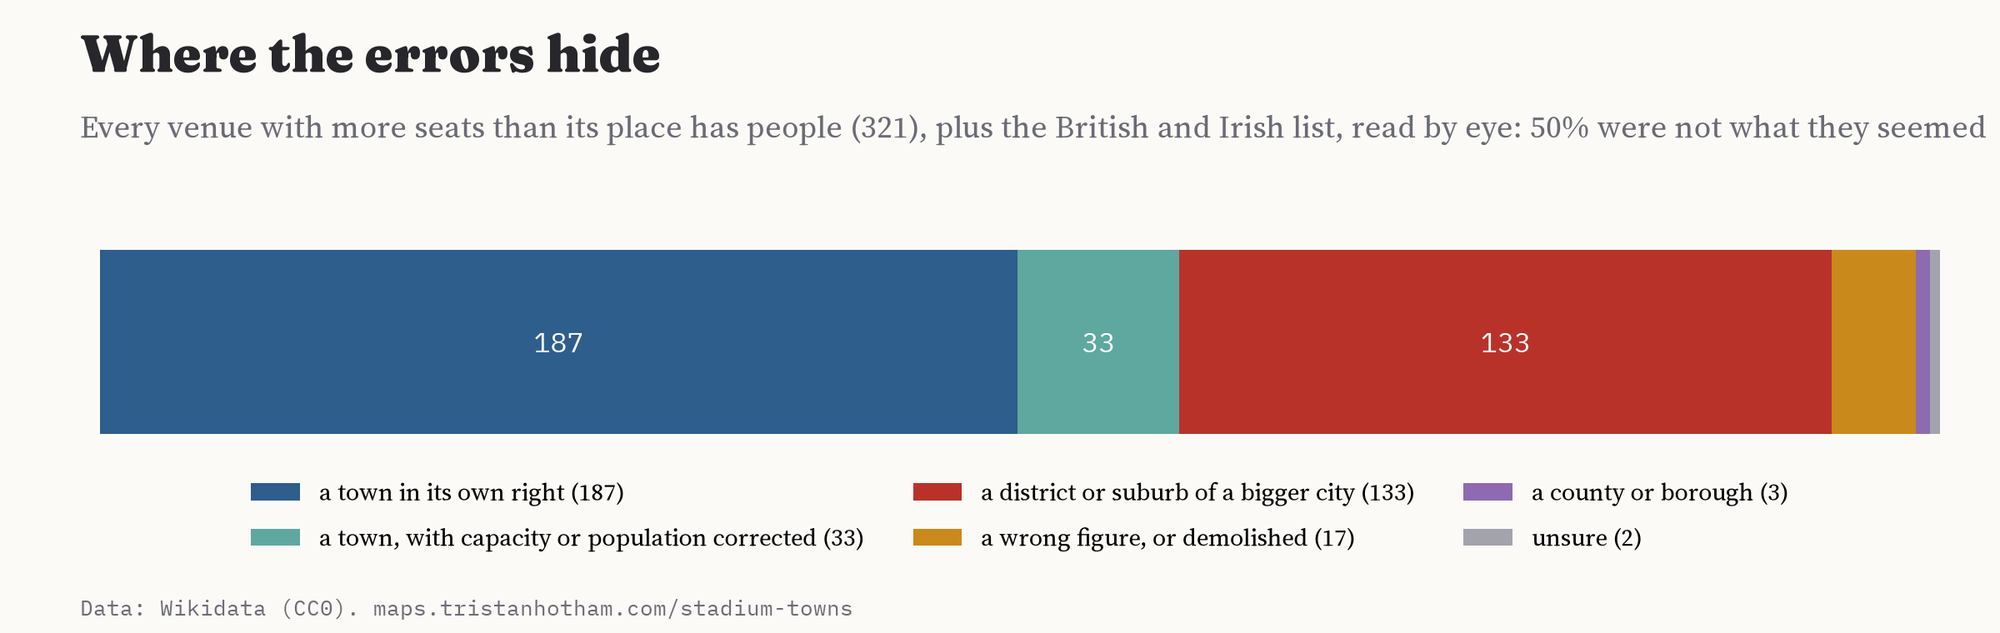
\includegraphics[width=\linewidth]{f_checks.png}\caption{Verdicts from reading every case at the head of the ranking.}\label{fig:checks}\end{figure}

\section{Limitations}
Outside the cases checked by hand, the largest recorded capacity can be an old standing record rather than today's seating, and the largest recorded population can be an old census peak (Pigadia's 630 is from an earlier census; the 2021 census counted 370); both are documented choices, not the only possible ones. Some capacities include standing room or banks (the 40,000 of Howard J. Lamade Stadium includes its hillside). Demolished venues stay in Wikidata; those found among the top cases were removed, but some may remain lower down. Irish populations are from the 2022 census, others from whatever year Wikidata records. Administrative populations vary in meaning between countries: a township, a commune and a census-designated place are not the same kind of town. The kind of venue and the sport are guessed from names. Venues below 1,000 seats, and venues not typed as sports venues in Wikidata, are absent. The country totals depend on how completely each country's venues are recorded. Cases with a ratio below 1 outside Britain and Ireland were not read by eye.

\section{Conclusion}
Stadiums bigger than their towns are real but rarer than a raw query suggests: half of the cases at the head of the ranking were artefacts of where Wikidata places a venue or needed a corrected figure. The true cases cluster in a few settings: American college and suburban stadiums, Irish county grounds, football grounds built just outside a city's boundary, and venues that fill for one race, one ski championship or one festival a year.

\section*{Data and code availability}
The interactive map is at \url{https://maps.tristanhotham.com/stadium-towns/}. Code, the overrides and the derived tables are at \url{https://github.com/Tristan-Hotham/stadium-towns} and archived with this paper at https://doi.org/10.5281/zenodo.24087795. Venue data are from Wikidata (CC0); Irish town populations from the Central Statistics Office; Natural Earth is public domain; text and figures CC BY 4.0; code MIT.

\section*{AI statement}
I wrote the text, with drafting and editing assistance from Claude (Anthropic), which also helped prepare the analysis code. I reviewed and checked all text and results.

\begin{thebibliography}{10}
\bibitem[Bast and Buchhold(2017)]{bast2017} Bast, H. and Buchhold, B. (2017) QLever: a query engine for efficient SPARQL+Text search. \textit{Proceedings of the 2017 ACM on Conference on Information and Knowledge Management (CIKM)}, 647 to 656. doi:10.1145/3132847.3132921.
\bibitem[Central Statistics Office(2023)]{cso2022} Central Statistics Office (2023) Census of Population 2022. Cork: Central Statistics Office.
\bibitem[Natural Earth(2026)]{naturalearth} Natural Earth (2026) Free vector and raster map data at 1:10m, 1:50m and 1:110m scales. \url{https://www.naturalearthdata.com/}.
\bibitem[Vrandečić and Krötzsch(2014)]{vrandecic2014} Vrandečić, D. and Krötzsch, M. (2014) Wikidata: a free collaborative knowledgebase. \textit{Communications of the ACM} 57(10), 78 to 85.
\end{thebibliography}
\end{document}
